%%%%%%%%%%%%%%%%%%%%%%%%%%%%%%%%%%%%%%%%%%%%%%%%%%%%%%%%%%%%%%%%%%%%%%
%% Journal of Engineering and Applied Science (Springer Nature) submission.
%% Built on the official Springer Nature template (sn-jnl.cls).
%% Single self-contained manuscript source; generated tables are \input
%% from tables/ and figures are \includegraphics from figures/ (scripted, no
%% hand-edited result cells). Reference style: sn-basic (numbered, per JEAS).
%% Article type: Research Article in engineering model-evaluation reliability.
%%
%% Every result-bearing number is copied from a validated, immutable asset under
%% manuscript/ (asset_inputs.json / tables/*.tex) and is auditable via
%% manuscript/paper-jeas/claim_ledger.jsonl + validate_jeas.py. No model was
%% refit, no result invented, no DOI minted, nothing submitted.
%%%%%%%%%%%%%%%%%%%%%%%%%%%%%%%%%%%%%%%%%%%%%%%%%%%%%%%%%%%%%%%%%%%%%%
\documentclass[pdflatex,sn-basic,Numbered]{sn-jnl}

\usepackage{graphicx}%
\usepackage{multirow}%
\usepackage{array}%
\usepackage{microtype}%
\usepackage{amsmath,amssymb,amsfonts}%
\usepackage{booktabs}%
\usepackage{url}%
\usepackage{setspace}%
\usepackage{lineno}%

\graphicspath{{figures/}}
\doublespacing
\linenumbers
\AtBeginDocument{%
  \hypersetup{bookmarksdepth=2}%
}

\begin{document}

\title[Reliable comparison of severe felt-intensity classifiers]{Reliable
comparison of severe felt-intensity classifiers with versioned and dependent
event data: a USGS DYFI benchmark}

\author*[1]{\fnm{Akshay} \sur{Sharma}}\email{akssha74@gmail.com}

\author[1]{\fnm{Lalji} \sur{Prasad}}\email{lalji.research@gmail.com}

\affil*[1]{\orgdiv{Department of Computer Science and Engineering},
\orgname{SAGE University}, \orgaddress{\city{Indore}, \postcode{452020},
\state{Madhya Pradesh}, \country{India}}}

\abstract{Engineers comparing classifiers on evolving event catalogues can reach
false conclusions when related events cross data splits or small score gaps are
treated as wins. We test whether classifiers of severe felt intensity
(event-maximum community decimal intensity $\geq6$) follow fixed input and
evaluation rules and whether their gains remain supported under a fixed
catalogue, event grouping, temporal holdout, and paired uncertainty.
From a frozen USGS ``Did You Feel It?'' (DYFI) snapshot of 7{,}520 $M\geq5$
records, we formed 2{,}362 eligible events, held out 430 events from 2023--2024,
and compared fixed baselines with Brier score and bootstrap intervals that
resampled whole event sequences. All four learned
models---magnitude-only and magnitude-plus-depth logistic regression, random
forest, and XGBoost---improved on the constant-prevalence reference. Adding
depth to the magnitude-only logistic model reduced Brier score by 0.018 (95\% CI
0.010--0.025). The magnitude-plus-depth logistic model and XGBoost both had
Brier 0.181 to three decimals, and their direct comparison remained unresolved.
The source-only input rule excluded a candidate using event year. A complementary
random-forest diagnostic gave similar point performance when related events were
kept together or split randomly; without an interval, we report it
descriptively.
The benchmark helps engineers reject inadmissible comparisons and unsupported
winner claims. It supports retrospective comparison; confirmation or operational
use requires fresh hidden data and separate validation.}

\keywords{model comparison, evaluation reliability, benchmark qualification,
dependent-event data, reproducibility, USGS DYFI}

\maketitle

\section{Introduction}\label{sec:intro}

Engineering model selection depends on comparisons that remain valid when a
dataset is updated, observations are dependent, and leading scores are close.
Without those controls, an apparent improvement can be caused by a changed
population, a proxy for the outcome or evaluation axis, cross-split dependence,
or unquantified sampling variation rather than by a better model. Standard
benchmarking is valuable precisely because it fixes a common task and metrics;
recent work in this journal, for example, compares object detectors on COCO to
support model selection for engineering applications~\citep{tian2024coco}.
The reliability problem is harder for event catalogues because both the
catalogue and the dependence structure can evolve.

The U.S. Geological Survey ``Did You Feel It?'' (DYFI) system is a useful
engineering case study. It converts crowdsourced felt reports into a
community-decimal intensity (CDI) for each earthquake and is widely reused as
an interpreted data product~\citep{wald1999dyfi,atkinson2007dyfi,wald2012dyfi,
quitoriano2020dyfi}. The target studied here is retrospective classification of
whether event-maximum CDI reaches 6 from outcome-blind source metadata. It is
not a real-time alert, causal model, or operational triage rule.

Our engineering question is: \emph{do performance and model-superiority claims
remain supportable when catalogue version, dependent-event splitting, temporal
evaluation, paired uncertainty, and reconstruction are controlled?} The
intended users are applied machine-learning engineers evaluating a candidate
classifier, maintainers publishing a stable benchmark, and reviewers auditing a
claimed improvement. They need two decisions: whether a candidate is admissible
for comparison and whether its improvement over a declared reference is
supported rather than a point-score fluctuation. Existing felt-intensity studies
use random or stratified partitions and do not provide that reusable decision
contract~\citep{patelli2026macroseismic,mori2025explainable}.

\subsection{Contributions}\label{sec:contrib}

We address unreliable model comparison by releasing a versioned benchmark and
an executable candidate-qualification contract. Concretely, the work provides:

\begin{enumerate}
\item \textbf{A versioned DYFI benchmark} with a dated, fingerprinted catalogue
snapshot, outcome-independent sequence grouping, and a fixed temporal holdout
(Sections~\ref{sec:data}--\ref{sec:roles}).
\item \textbf{An auditable candidate test} that checks allowed inputs and role
isolation before scoring, then uses fixed baselines and paired Brier uncertainty
to decide whether an improvement is supported
(Sections~\ref{sec:leakage}--\ref{sec:qualification}).
\item \textbf{A worked model-selection example} showing a clear gain from depth
beyond magnitude alone, a competitive transparent logistic reference, and the
point at which a more complex model remains unresolved. Data, frozen parameters,
tests, and prediction-reconstruction records are released with the benchmark
(Section~\ref{sec:results}).
\end{enumerate}

The primary contribution is the benchmark and its comparison process, not a new
production classifier.

\subsection{Engineering significance and intended use}\label{sec:significance}

The output is an engineering test harness for transparent retrospective model
comparison. A declared candidate enters through the released schema, is
excluded if it uses forbidden outcome-derived fields or violates role
isolation, is scored on the fixed temporal holdout, and is compared with paired
sequence-cluster uncertainty. This workflow prevents an engineer or reviewer
from declaring superiority from a different catalogue version, a contaminated
split, or an unresolved point difference. Because holdout labels are public,
the release is not an untouched prospective test: confirmatory evaluation of a
new model requires a fresh benchmark version or hidden evaluation service.
Table~\ref{tab:engineering-failures} names the failure prevented by each
control, and Fig.~\ref{fig:qualification-workflow} shows the decision path.

% GENERATED by build_utility_assets.py -- do not edit.
\begin{table*}[t]
\centering
\small
\caption{Engineering failure modes addressed by the benchmark qualification contract}
\label{tab:engineering-failures}
\begin{tabular}{p{0.20\textwidth}p{0.28\textwidth}p{0.34\textwidth}}
\toprule
Failure source & Invalid engineering conclusion & Qualification control \\
\midrule
Catalogue revision & Non-identical event population & Frozen access instant + SHA-256 release \\
Outcome-derived field & Label leakage & F1/F2 schema audit \\
Identifier or downstream proxy & Proxy leakage & F3/F4 field audit \\
Sequence crosses roles & Dependent-event contamination & F5 sequence-role audit \\
Temporal-cutoff violation & Future information in development & F6 temporal audit \\
Point-score ranking & False model-superiority claim & Paired sequence-cluster interval \\
Environment drift & Irreproducible scores/artifacts & Pinned environment + reconstruction hash \\
\bottomrule
\end{tabular}
\end{table*}


\begin{figure*}[t]
\centering
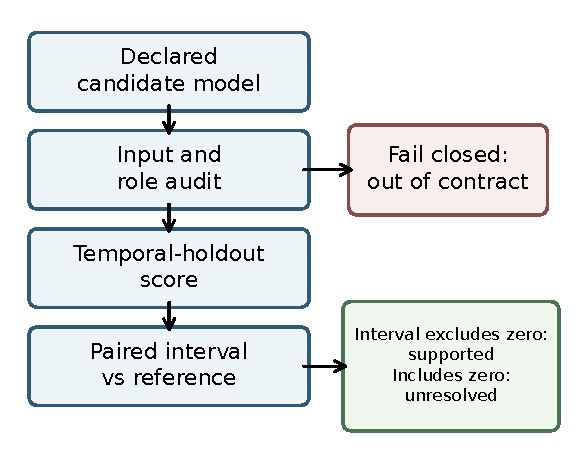
\includegraphics[width=0.82\textwidth]{fig_candidate_workflow.pdf}
\caption{\textbf{Candidate-model qualification.} A candidate that fails the
schema, proxy, role, or temporal audit is inadmissible. An admitted candidate is
scored on the fixed holdout and compared with paired uncertainty; an interval
including zero remains unresolved rather than becoming a winner claim}
\label{fig:qualification-workflow}
\end{figure*}

\section{Related work and novelty}\label{sec:related}

\paragraph{DYFI and reusable macroseismic data.}
Foundational DYFI work defines community decimal intensity, quality control,
response dependence, and post-event revision~\citep{wald1999dyfi,
atkinson2007dyfi,wald2012dyfi,quitoriano2020dyfi}.
\citet{rosler2022documentation} therefore recommend preserving timestamped
interpreted products. Related resources include INGe and the Western North
America macroseismic release~\citep{oliveti2022inge,fathiansabet2026western},
historical databases~\citep{neefs2025btm,sira2025macrosisdata}, and
crowdsourced analyses of shaking and geology~\citep{kouskouna2021athens,
sarao2023crowdsourcing}. These works motivate a frozen, reusable evaluation
resource but do not define the present event-level classification contract.

\paragraph{Machine-learning and engineering comparisons.}
Felt-intensity models have used random forests or boosting with instrumental,
catalogue, or crowdsourced predictors~\citep{lilienkamp2023feltreports,
patelli2026macroseismic,mori2025explainable,ozupak2026alert,
ertuncay2025detection}. The closest same-source study uses a naive split for
DYFI regression~\citep{kumar2025dyfiindia}; a concurrent DYFI benchmark studies
per-location MMI simulation and identifier leakage~\citep{li2025llmworldmodels}.
EarthquakeNPP supplies the nearest broader leakage-aware seismological benchmark
but targets occurrence forecasting~\citep{stockman2026earthquakenpp}.
JEAS precedents demonstrate decision-oriented benchmark and model comparisons in
object detection, rock properties, and pavement maintenance
~\citep{tian2024coco,niu2024ucs,alnaqbi2025pavement}, while seismic engineering
work makes the affected response and design interpretation explicit
~\citep{seleemah2022bridge}. The present study adopts that decision-oriented form
for model-comparison reliability rather than proposing a new classifier.

\paragraph{Evaluation-method delta.}
Grouped or blocked validation for dependent data and leakage prevention are
established principles~\citep{roberts2017cv,kaufman2012leakage}. The delta is
the released combination for this task: a timestamped and hashed single-source
corpus, executable feature/proxy and split audits, outcome-independent
sequence-grouped roles, a temporal holdout, fixed baselines, paired
sequence-cluster uncertainty, and exact reconstruction. No individual component
is claimed as new; the contribution is the auditable engineering comparison
contract and its worked decision example.

\section{Data, provenance, and outcome-boundary disclosure}\label{sec:data}

\paragraph{Source and single-instant pinning.} The corpus is derived entirely
from USGS DYFI and its parent ANSS Comprehensive Catalog (ComCat), retrieved
through the International Federation of Digital Seismograph Networks (FDSN)
event web service~\citep{usgs_dyfi_data,usgs_comcat}. The
acquisition envelope is outcome-independent: $M\geq5$, product type
\texttt{dyfi}, event type \texttt{earthquake}, starttime 2015-01-01 to endtime
2025-01-01. FDSN defines the end bound as inclusive; no frozen record occurs
at that boundary, so the realized snapshot spans 2015--2024. Results are ordered
by time. Because the catalogue evolves, the data were frozen at one access
instant (2026-09-01T06:33:30Z) and assigned a SHA-256 fingerprint. Preliminary
counts changed from 7{,}575 to 7{,}576 during acquisition, documenting a live
catalogue revision. The final payload contained 7{,}520 records, and a count
requested 50 seconds later also returned 7{,}520. The earlier counts had no
paired payload, so their membership differences cannot be decomposed and are
recorded as provenance, not analysis exclusions. The downloaded bytes and their
fingerprint define this resource version
(Table~\ref{tab:cohort}, Fig.~\ref{fig:cohort}).

\paragraph{Protocol chronology.} The file records an internal 2026-09-01 freeze
but was first publicly timestamped on 2026-09-19. We therefore describe it as an
internally frozen protocol, not an externally registered preregistration.

\paragraph{Retrospective eligibility and post-report ascertainment.} DYFI
intensity is an after-the-event quantity whose reliability grows with the number
of felt reports~\citep{quitoriano2020dyfi}. To keep the label meaningful we apply
a data-informed eligibility filter of at least ten responses per event. The
response count is used \emph{only} for eligibility and is explicitly forbidden as
a predictive feature, because it is a post-outcome ascertainment proxy; this
forbiddance is enforced by the leakage audit (family F2,
Section~\ref{sec:leakage}). Eligibility yields 2{,}362 events with severe
prevalence 0.298 (703 severe events). Of these, 2{,}360 events are assigned to
the internally specified analysis roles (Section~\ref{sec:roles}) and contain 702 severe
events; the remaining two are temporal-straddle exclusions, one of which is
severe. That single severe straddle event accounts for the difference between the
eligible cohort (703 severe) and the analysis-assigned set (702 severe), so
eligibility is not the same as analysis-role assignment (Table~\ref{tab:cohort}).

\paragraph{Endpoint.} We label an event severe when its event-maximum CDI is at
least 6.0 (intensity VI or greater). We use 6.0 as the primary threshold and
report sensitivity at 5.5, 6.0, and 6.5. We also examine a near-threshold band
of $\pm0.5$ (Section~\ref{sec:endpoint-results}).

\paragraph{Outcome-boundary disclosure and held-out semantics.} Only corpus-level
outcome-blind counts and inherited aggregate feasibility statistics were exposed
before construction; no per-event label informed the endpoint, split, or
tuning choices, and role membership is assigned by an internally specified,
outcome-independent rule that never uses the label. We therefore describe the
external holdout as \emph{held out from model development with aggregate
feasibility previously known}, and we deliberately do \emph{not} call it
``untouched'' or ``confirmatory.'' Two event identifiers were prelisted for
quarantine because their aggregate counts had been seen during source
verification; neither identifier occurs in the frozen snapshot, so the rule is
non-operative in version~1 and excludes no record. The complete list of protocol decisions is reported in
Section~\ref{sec:repro-results}. No
respondent-level personally identifying information is redistributed; only
event-level source metadata, the severe label, the eligibility-only response
count, identifiers, and role assignments are released. Snapshot-level
provenance is supplied by the activated source-locator manifest and source
payload SHA-256; version~1 does not claim per-event product-version hashes. The
release bundle follows datasheet-for-datasets
documentation~\citep{gebru2021datasheets} and findable, accessible,
interoperable, and reusable (FAIR) data
principles~\citep{wilkinson2016fair}.

\section{Benchmark design}\label{sec:design}

\subsection{Feature sets and the six-category leakage audit}\label{sec:leakage}

The primary \emph{source-only} feature set contains magnitude and depth. It is
the only feature set evaluated on the temporal holdout. An
\emph{expanded-metadata} sensitivity analysis (baseline B3) additionally uses
latitude, longitude, and event year. Event year is known at prediction time and
is not intrinsically label leakage, but it is excluded by the declared
source-only temporal-holdout contract. The audit accepts only an approved
feature set with the expected fields in the expected order; any extra or unknown
field is rejected.

The executable audit enforces six leakage families. Field-level: F1 direct
label or its constituents; F2 post-outcome ascertainment or revision (including
the response count, eligibility-only); F3 identifier or source proxy; F4
downstream-product proxy. Split-level: F5 sequence cross-role straddle; F6
temporal-cutoff violation. An axis-variable check additionally rejects origin year
under a temporal holdout and, when a geographic holdout is configured,
latitude/longitude/region. The latter audit branch is provided for reuse but was
not executed as an external evaluation in this study. This enforces a
conservative B3 scope restriction; it is not evidence that event year is a
leaking label proxy. The audit is useful independently of
model performance: it must reject every deliberately contaminated test case and
accept only the approved clean feature set. It is exercised by 110 unit tests
across four suites, all passing, and accepted the source-only feature set in the
frozen snapshot.

\subsection{Sequence grouping and outcome-independent roles}\label{sec:roles}

Events are grouped into seismic \emph{sequences} by order-stable single-link
space--time connected components (100~km, 30~days); the sequence, not the event,
is the unit of role assignment, so events linked by this fixed rule cannot
straddle roles. This rule is a deterministic grouping heuristic, not a validated
catalogue of all physical mainshock--aftershock relationships; unlinked true
aftershocks may therefore remain in different roles. Roles are
assigned by an internally specified, outcome-independent rule (fixed assignment key,
temporal cutoff year 2023, development fraction 0.2, five cross-validation
folds); the rule provably never reads the label. The external holdout contains
events on or after 2023. The frozen internal protocol also named a secondary
leave-region-out geographic evaluation, but that branch was not executed and no
geographic role manifest is claimed. The reported geographic result instead
summarizes the temporal-holdout predictions by 10$^\circ$ cell
(Supplementary Table~S3); Supplementary Table~S2 records this deviation.
Digital fingerprints of the completed temporal role assignments are published
so that third parties can verify them. The
partition is exhaustive and disjoint:
$1{,}573+357+430+2=2{,}362$ events, comprising 1{,}573 train, 357 development,
430 external temporal holdout, and 2 temporal-straddle exclusions
(Table~\ref{tab:cohort}, Fig.~\ref{fig:cohort}). Construction (train plus
development) is 1{,}930 events across 1{,}530 sequences; the holdout is 430
events across 354 sequences.

\subsection{Baseline suite and exclusions}\label{sec:baselines}

The fixed suite is B0 no-skill (constant prevalence), B1 magnitude-only logistic
regression, B2 source-only logistic regression, B3 expanded-metadata logistic
regression (used only in compatible sensitivity analyses), B4 random forest
(scikit-learn;
\citealp{pedregosa2011sklearn}), and B5 XGBoost~\citep{chen2016xgboost}. Each learned
baseline is tuned \emph{only} by the protocol-defined deterministic grouped
cross-validation on the construction corpus over a fixed grid, named before
evaluation, and carried unchanged to the protected holdout with frozen
best parameters. A machine-readable fit log enforces a maximum of 120 model
fits; the executed run used 91. Two comparators are excluded for protocol-defined,
reproducible reasons recorded in the protocol-decision table
(Section~\ref{sec:repro-results}): B3 is not evaluated on the temporal holdout
because origin year is outside the declared source-only feature contract; and
the Atkinson--Wald (2007) DYFI intensity-prediction
equation~\citep{atkinson2007dyfi} is excluded because it cannot be applied to
the source-only feature set and tectonically heterogeneous population without
inventing a site-distance covariate, a per-event tectonic-regime assignment, and
a probability link.

\subsection{Metrics, calibration, uncertainty, and ranking}\label{sec:metrics}

The primary score is the Brier score~\citep{brier1950}; secondary scores are
log-loss, AUROC, and calibration intercept/slope~\citep{vancalster2019calibration}.
For numerical stability, log-loss clips predicted probabilities symmetrically
to $[10^{-15},1-10^{-15}]$ before taking logarithms.
Brier-score uncertainty is quantified by a sequence-cluster bootstrap
($n_{\text{boot}}=2000$, 95\% intervals) that resamples whole sequences rather
than events~\citep{field2007bootstrap}, with a minimum-valid-replicate rule.
Calibration and feasibility states are \emph{derived}, not hard-coded: a
constant-prevalence predictor has no identifiable calibration slope, so the
table reports that value as unavailable. Pairwise ranking uses a paired
sequence-cluster bootstrap Brier difference with an explicit tie probability;
the table reports whether each 95\% interval includes zero, together with a
tie-aware joint ordering (Section~\ref{sec:pairwise-results}). Because the
intervals use 2{,}000 Monte Carlo draws, near-zero endpoints are interpreted
cautiously rather than as stable ranking guarantees.
The protocol requested intervals for every metric; only Brier-based intervals
were retained, so other metrics are descriptive point estimates
(Supplementary Table~S2).

\subsection{Protected evaluation and reproducibility}\label{sec:oneshot}

The official decision-bearing protected evaluation was authorized once by an
automated, globally consumed token; the one-shot wrapper refuses a second
authorized run. After the result was fixed, the token-free deterministic
analytic core was replayed twice, reproducing the recorded result fingerprint
exactly. Thus, single-use refers to result authorization, not later verification.
The frozen holdout predictions were also recovered bit-for-bit from the released
rows and best parameters under a pinned scientific-Python environment (NumPy,
SciPy, scikit-learn, XGBoost;
\citealp{harris2020numpy,virtanen2020scipy,pedregosa2011sklearn,chen2016xgboost}).
All fits, exclusions, subsets, cutoffs, and pairwise comparisons are reported
regardless of outcome; the only permitted omissions are the protocol-defined
exclusions above.
Computation is local-only under a pinned environment.

\paragraph{Reproducible artwork and generative AI assistance.} All figures were
generated with Matplotlib~3.11.1 directly from the frozen analysis assets; no
manual image manipulation or AI-generated artwork was used. ChatGPT assisted
language editing, formatting, code review, literature discovery, and revision
suggestions. It did not generate data, run model fits, or create the reported
results. The authors verified all sources, computations, interpretations, and
assisted changes and retain full responsibility.

\section{Results}\label{sec:results}

All result-bearing values below are generated from the frozen analysis outputs
and checked automatically against their source records; no result cell was
hand-edited.

\subsection{Cohort and roles}\label{sec:cohort-results}

Table~\ref{tab:cohort} and Fig.~\ref{fig:cohort} give the cohort accounting. Of
7{,}520 frozen DYFI records, 2{,}362 events pass the ten-response eligibility
filter (severe prevalence 0.298; 703 severe events), partitioned into 1{,}573
train, 357 development, and a 430-event temporal holdout, with two
temporal-straddle exclusions. Thus 2{,}360 of the 2{,}362 eligible events receive
analysis roles; they contain 702 severe events, and the 703rd severe event is one
of the two straddle exclusions. Two identifiers prelisted for quarantine are
absent from the frozen snapshot, so that safeguard removes no version~1 record.
Construction severe prevalence is 0.285 and
holdout prevalence is 0.351; the higher holdout prevalence reflects the temporal
transport shift and is reported, not adjusted.

\begin{figure*}[t]
\centering
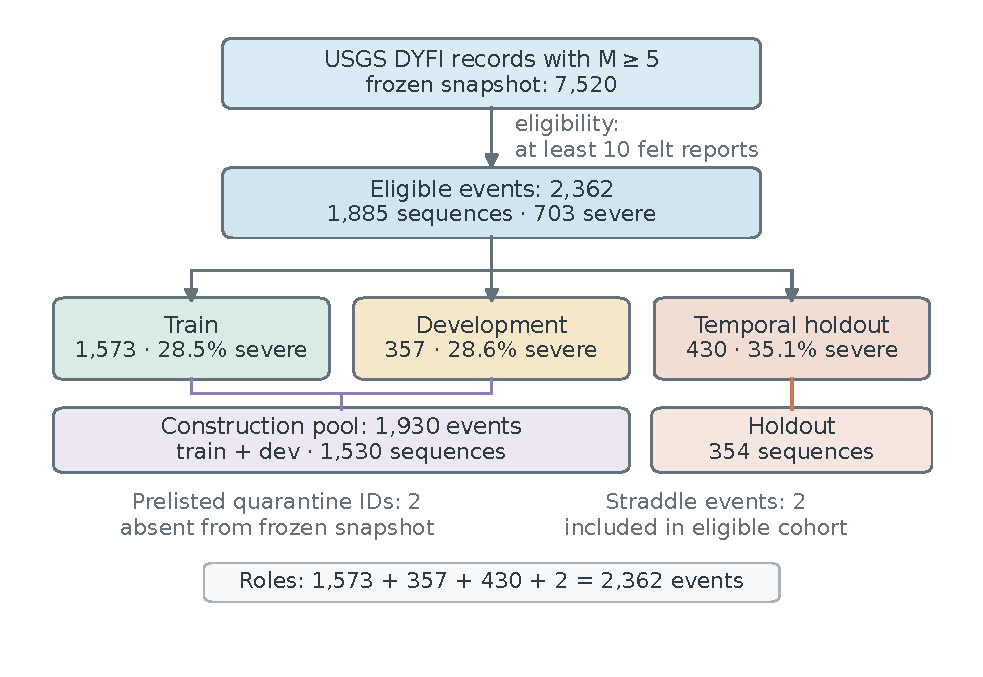
\includegraphics[width=\textwidth]{fig_cohort_flow.pdf}
\caption{\textbf{Cohort construction and role assignment.} On the
frozen USGS DYFI $M\geq5$ snapshot. The 7{,}520 source records yield 2{,}362
eligible events in 1{,}885 seismic sequences. Of these, 2{,}360 are assigned to
train ($n=1{,}573$), development ($n=357$), or temporal holdout ($n=430$);
two straddle events are excluded from role assignment}
\label{fig:cohort}
\end{figure*}

% GENERATED by manuscript/code/build_tables.py -- do not edit by hand.
\begin{table*}[t]
\centering
\small
\caption{Cohort accounting and outcome-independent role assignment}
\label{tab:cohort}
\resizebox{\textwidth}{!}{%
\begin{tabular}{lrrrr}
\toprule
Stage & Events & Severe & Severe rate & Sequences \\
\midrule
USGS DYFI records with $M\geq5$ (frozen snapshot) & 7520 & -- & -- & -- \\
Eligible (at least 10 felt reports) & 2362 & 703 & 0.298 & 1885 \\
\quad Train & 1573 & 449 & 0.285 & -- \\
\quad Development & 357 & 102 & 0.286 & -- \\
\quad Construction (train+dev) & 1930 & 551 & 0.285 & 1530 \\
\quad External temporal holdout & 430 & 151 & 0.351 & 354 \\
Temporal-straddle excluded & 2 & 1 & -- & 1 \\
\bottomrule
\end{tabular}
}%

\par\vspace{2pt}\footnotesize\emph{Note.} Roles were fixed without using outcomes. Two event identifiers prelisted for quarantine are absent from the frozen snapshot, so the safeguard removes no version~1 record. Severe $=1$ when an event's maximum community decimal intensity (CDI) is at least 6. The eligible severe count reconciles as 703 = 449 (train) $+$ 102 (development) $+$ 151 (holdout) $+$ 1 (straddle exclusion). Thus the 2360 role-assigned events contain 702 severe events.
\end{table*}


\subsection{Difficulty and endpoint sensitivity}\label{sec:endpoint-results}

Table~\ref{tab:threshold} and the left panel of Fig.~\ref{fig:threshold} report a
descriptive fixed-prediction threshold probe. As the severe cut moves from
5.5 to 6.5, holdout prevalence falls smoothly (0.458, 0.351, 0.260) and the
source-only logistic-regression Brier score and AUROC move monotonically (Brier
0.240, 0.181, 0.143;
AUROC 0.734, 0.786, 0.815). On the construction corpus the near-threshold
fraction ($|\mathrm{maxCDI}-6|<0.5$) is 0.164 and the no-skill Brier score is
0.204, bounding the difficulty of the primary endpoint. This probe relabels and
rescores probabilities fitted for the primary 6.0 endpoint; it does not refit
or recalibrate B2 at 5.5 or 6.5 and therefore does not establish endpoint
robustness. The protocol-required aggregation-grid sensitivity was
not executed and is disclosed as a deviation (Supplementary Table~S2).

\begin{figure*}[t]
\centering
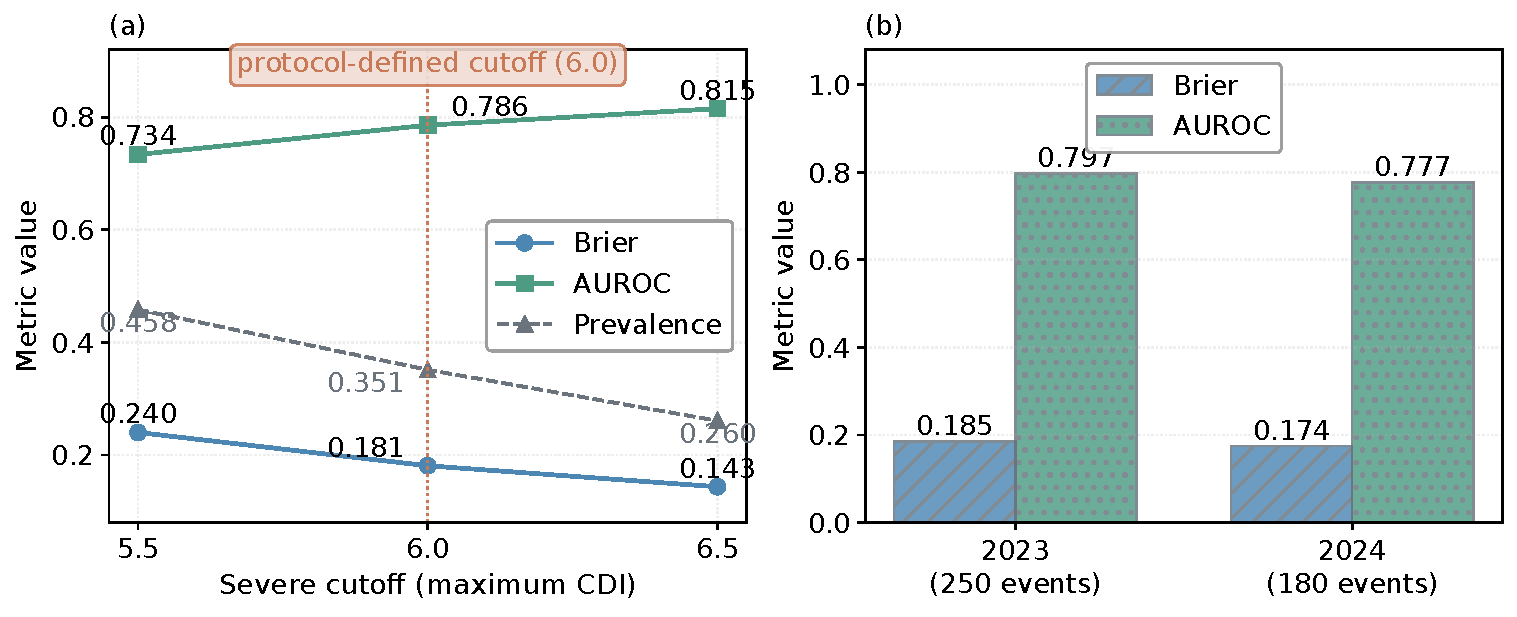
\includegraphics[width=\textwidth]{fig_threshold_slice.pdf}
\caption{\textbf{Endpoint and temporal sensitivity.} Results for the source-only logistic regression (B2).
(a) Performance as the severe-intensity cutoff varies. (b) Performance
within the 2023 ($n=250$) and 2024 ($n=180$) portions of the temporal holdout.
The cutoff analysis rescores fixed B2 probabilities without refitting. Lower
Brier score and higher AUROC are better}
\label{fig:threshold}
\end{figure*}

% GENERATED by manuscript/code/build_tables.py -- do not edit by hand.
\begin{table*}[t]
\centering
\small
\caption{Endpoint-threshold probe using fixed source-only probabilities}
\label{tab:threshold}
\begin{tabular}{lrrr}
\toprule
Maximum CDI cutoff & Severe rate & Brier score & AUROC \\
\midrule
5.5 & 0.458 & 0.240 & 0.734 \\
6.0 $^a$ & 0.351 & 0.181 & 0.786 \\
6.5 & 0.260 & 0.143 & 0.815 \\
\bottomrule
\end{tabular}
\par\vspace{2pt}\footnotesize\emph{Note.} $^a$~Protocol-defined primary cutoff ($\geq 6$). CDI denotes community decimal intensity. The sensitivity rows relabel and rescore fixed B2 probabilities; B2 is not refit or recalibrated for the alternate cutoffs. In the construction sample, 0.164 of events lie within 0.5 CDI units of the primary cutoff, and the no-skill Brier score is 0.204. Lower Brier score and higher AUROC indicate better performance.
\end{table*}


\subsection{Complementary split-assignment diagnostic}\label{sec:leakage-results}

As a secondary stress test, we compare naive random and sequence-grouped folds
for a fixed random forest with 300 trees and unrestricted depth under three
fold-assignment schemes on the construction corpus
(Table~\ref{tab:leakage}, Fig.~\ref{fig:leakage}).
This diagnostic asks whether split assignment changes point performance in this
corpus; it is not the qualification workflow's decision-bearing result. It is
also distinct from the tuned temporal-holdout baseline B4, whose maximum depth
is 3.
On this $M\geq5$
one-row-per-event universe the point estimates are small and slightly reversed:
sequence grouping produced a Brier score 0.0059 lower and an AUROC 0.0124
higher than random-event splitting, calculated from unrounded
scores. The sequence-grouped split therefore scores marginally \emph{better}
than the naive random split, not worse. The frozen internal protocol required
uncertainty reporting for this contrast but did not define a paired interval
estimator; the executed result contains point estimates only. We disclose this
unfulfilled element as a deviation and do not invent a post-hoc interval.
Accordingly, we report the contrast descriptively, not as
evidence of equivalence, a true zero effect, leakage, or a win. Its
plausible structural context is that 1{,}885 sequences are largely singleton
(1{,}530 in construction), leaving limited within-sequence near-duplicate
structure for a random split to leak. This does not prove a small true effect.
With one row per event,
event grouping imposes the same grouping constraint as random-event assignment,
but its deterministic fold allocation differs and therefore produces different
scores. It is reported as an intermediate control. The protocol remains reusable on datasets with more
multi-event sequences. The present result neither demonstrates practically
important leakage from random splitting nor establishes its absence.

\begin{figure*}[t]
\centering
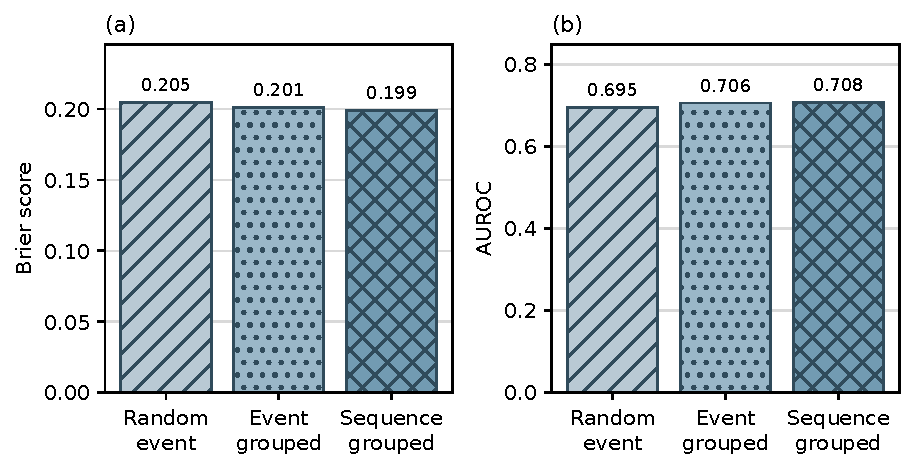
\includegraphics[width=\textwidth]{fig_split_diagnostic_jeas.pdf}
\caption{\textbf{Split-assignment diagnostic.} Five-fold performance of the fixed diagnostic (random forest:
300 trees, unrestricted depth) under random-event, event-grouped, and
sequence-grouped fold assignment in the construction sample. Relative to
random-event splitting, sequence grouping produced (a) a Brier score 0.0059
lower and (b) an AUROC 0.0124 higher. The diagnostic is distinct from tuned temporal-holdout
baseline B4. The small, reversed differences provide no evidence of performance
inflation from random splitting in this sample. Both axes start at zero}
\label{fig:leakage}
\end{figure*}

% GENERATED by manuscript/code/build_tables.py -- do not edit by hand.
\begin{table*}[t]
\centering
\small
\caption{Split-assignment performance of the fixed diagnostic}
\label{tab:leakage}
\begin{tabular}{lrrrr}
\toprule
Fold assignment & Brier score & AUROC & Log-loss & Folds \\
\midrule
Random-event (naive) & 0.2048 & 0.6952 & 0.9640 & 5 \\
Event-grouped (control) & 0.2009 & 0.7058 & 0.9223 & 5 \\
Sequence-grouped (primary) & 0.1990 & 0.7076 & 0.9709 & 5 \\
\bottomrule
\end{tabular}
\par\vspace{2pt}\footnotesize\emph{Note.} The diagnostic is distinct from the tuned temporal-holdout baseline B4 (depth 3). Using unrounded values, sequence grouping produced a Brier score 0.0059 lower and an AUROC 0.0124 higher than random-event splitting. The frozen internal protocol required uncertainty but did not define the paired interval estimator; the executed report retained point estimates only. This deviation is disclosed, and no post-hoc interval or equivalence claim is added. Because there is one row per event, event grouping imposes the same grouping constraint as random-event assignment, but its deterministic fold allocation is different and can produce different scores.
\end{table*}


\subsection{Baseline performance and calibration}\label{sec:baseline-results}

Table~\ref{tab:baselines} and Fig.~\ref{fig:baselines} give per-baseline holdout
performance ($n=430$) with sequence-cluster bootstrap 95\% intervals. The
no-skill B0 has Brier 0.232 ($[0.212,0.253]$); its calibration slope cannot be
estimated because it assigns the same probability to every event. The learned
baselines have lower Brier (B1 0.198,
B2 0.181, B4 0.187, B5 0.181) with overlapping intervals; calibration
intercept/slope pairs are finite and positive. B2 and B5 both round to the
lowest Brier score, 0.181; their paired comparison is reported in
Section~\ref{sec:pairwise-results}.

\begin{figure*}[t]
\centering
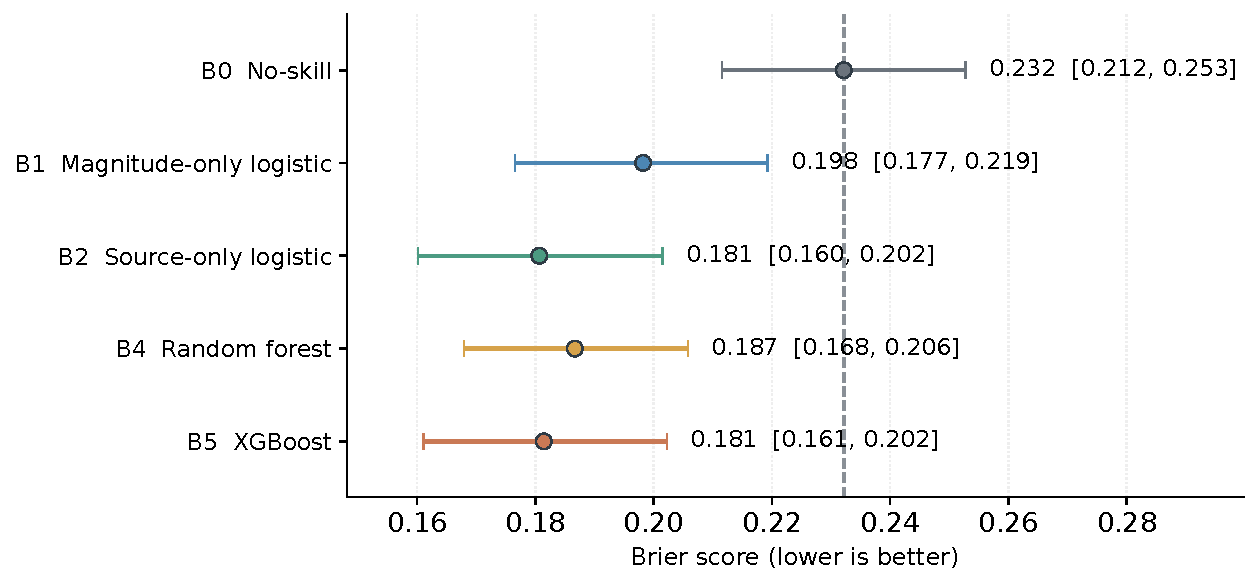
\includegraphics[width=\textwidth]{fig_baseline_scores.pdf}
\caption{\textbf{Temporal-holdout baseline performance.} Brier scores and 95\% sequence-cluster bootstrap confidence intervals
for the five baselines on the temporal holdout ($n=430$). Lower values are
better; the vertical dashed line marks the no-skill B0 score. B3 is omitted
because event year is outside the declared source-only temporal-holdout contract
(Supplementary Table~S2)}
\label{fig:baselines}
\end{figure*}

% GENERATED by manuscript/code/build_tables.py -- do not edit by hand.
\begin{table*}[t]
\centering
\small
\caption{Temporal-holdout performance of fixed baseline models}
\label{tab:baselines}
\setlength{\tabcolsep}{4.5pt}
\resizebox{\textwidth}{!}{%
\begin{tabular}{lccccc c}
\toprule
Baseline & Brier & 95\% CI & Log-loss & AUROC & Calibration$^a$ & Accuracy \\
\midrule
B0 (no-skill) & 0.232 & [0.212, 0.253] & 0.658 & 0.500 & INFEASIBLE & 0.65 \\
B1 (magnitude-only logistic) & 0.198 & [0.177, 0.219] & 0.583 & 0.719 & 0.32 / 1.02 & 0.70 \\
B2 (source-only logistic) & 0.181 & [0.160, 0.202] & 0.536 & 0.786 & 0.64 / 1.29 & 0.73 \\
B4 (random forest) & 0.187 & [0.168, 0.206] & 0.553 & 0.777 & 0.74 / 1.48 & 0.73 \\
B5 (XGBoost) & 0.181 & [0.161, 0.202] & 0.541 & 0.783 & 0.42 / 1.07 & 0.74 \\
\bottomrule
\end{tabular}
}%

\par\vspace{2pt}\footnotesize\emph{Note.} $^a$~Intercept / slope. These values cannot be estimated for B0 because it assigns the same probability to every event. B3 includes event year and is therefore omitted from the temporal holdout (Table~\ref{tab:exclusions}). Accuracy uses a fixed probability cutoff of 0.5 that was not selected on the holdout. Log-loss clips probabilities to $[10^{-15},1-10^{-15}]$. Lower Brier score and log-loss are better; higher AUROC and accuracy are better. The two lowest-Brier models cannot be distinguished in their direct paired comparison.
\end{table*}


\subsection{Worked candidate qualification}\label{sec:qualification}

Table~\ref{tab:qualification} applies the released engineering decision rule to
the six fixed candidates. B3 is outside the source-only contract because it
contains event year; this is a conservative scope exclusion, not demonstrated
label leakage. B1, B2, B4, and B5 pass the audit and each has a paired
Brier interval below the no-skill B0 reference. The contract therefore supports
their improvement over B0. The direct B2--B5 interval includes zero, so the
small point difference is not enough to prefer one model on Brier score. This
worked example demonstrates the benchmark's intended use: admit valid
candidates, identify supported improvements, and provide a clear reference
against which future methods can be tested.

% GENERATED by build_utility_assets.py -- do not edit.
\begin{table*}[t]
\centering
\small
\caption{Worked candidate-model qualification using the frozen temporal holdout}
\label{tab:qualification}
\resizebox{\textwidth}{!}{%
\begin{tabular}{p{0.25\textwidth}p{0.12\textwidth}p{0.17\textwidth}p{0.23\textwidth}p{0.16\textwidth}}
\toprule
Candidate & Audit gate & Holdout Brier [95\% CI] & Brier difference vs B0 [95\% CI] & Contract decision \\
\midrule
B0 no-skill & Pass (reference) & 0.232 [0.212, 0.253] & --- & Reference only \\
B1 magnitude-only logistic & Pass & 0.198 [0.177, 0.219] & -0.0339 [-0.0511, -0.0171] & Supported vs B0 \\
B2 source-only logistic & Pass & 0.181 [0.160, 0.202] & -0.0515 [-0.0681, -0.0342] & Supported vs B0 \\
B4 random forest & Pass & 0.187 [0.168, 0.206] & -0.0455 [-0.0598, -0.0307] & Supported vs B0 \\
B5 XGBoost & Pass & 0.181 [0.161, 0.202] & -0.0507 [-0.0682, -0.0319] & Supported vs B0 \\
B3 expanded-metadata logistic & Out of contract & --- & --- & Year excluded by source-only schema \\
\bottomrule
\end{tabular}
}%

\par\vspace{2pt}\footnotesize\emph{Decision rule.} A candidate is first admitted by the schema, proxy, role, and temporal audits. A lower paired Brier interval that excludes zero supports improvement over the declared reference; otherwise the comparison remains unresolved. All four learned baselines improve over B0. B2 versus B5 remains unresolved (B2$-$B5 -0.0008, 95\% CI [-0.0078, 0.0068]), so the contract prevents a false winner declaration.
\end{table*}


\subsection{Pairwise ranking stability}\label{sec:pairwise-results}

Supplementary Table~S1 reports all ten pairwise Brier-score comparisons. Every
learned baseline performs better than the no-skill reference B0 (all four
intervals exclude zero). The source-only logistic model B2 also improves on the
magnitude-only B1 by 0.0176 (95\% interval 0.0101--0.0249), showing that depth
adds useful predictive information in this dataset. XGBoost B5 improves on the
random forest B4, although the lower interval endpoint (0.0003) is near the
Monte Carlo boundary. We treat this contrast cautiously and do not use it as a
ranking certificate. The B2--B4 and B2--B5 comparisons have intervals that
include zero. In the joint
bootstrap ordering, B2 has the highest probability of being uniquely best
(0.613), followed by B5 (0.387), but the direct B2--B5 comparison remains
uncertain. The source-only logistic model therefore provides a strong,
transparent reference for future candidates, but the results do not justify
naming it a winner.

The frozen internal protocol allowed an ``equivalent'' verdict but did not specify a
positive numerical equivalence margin; its resolution floor was zero. We
therefore do not invent a post-hoc margin or label any models equivalent.
Instead, we report each point difference, 95\% interval, and
whether that interval includes zero. Supplementary Table~S2 records this
interpretive restriction, which changes no result.

\subsection{Temporal and geographic subgroup summaries}\label{sec:slices-results}

Supplementary Table~S3 and the right panel of Fig.~\ref{fig:threshold} report the
temporal and geographic subgroup summaries for the source-only logistic
regression within the temporal holdout. The two
holdout years are internally consistent (2023: $n=250$, Brier 0.185, AUROC 0.797;
2024: $n=180$, Brier 0.174, AUROC 0.777). The geographic subgroup summary spans
82 occupied $10^\circ$ cells (per-cell Brier 0.002--0.825, median 0.151).
These values stratify the same 430 temporal-holdout predictions; they are not a
leave-region-out evaluation and support no geographic or cross-system
generalization claim.

\subsection{Exclusions, deviations, and reproducibility}\label{sec:repro-results}

Supplementary Table~S2 explains the protocol decisions most relevant to
interpretation: excluded comparators and records, the unexecuted geographic
transport branch, the unfulfilled split-contrast interval, and the absence of an
equivalence claim. The tagged public release contains the complete SHA-256
fingerprints, software environment, and machine-readable verification details.
Its public-release manifest fingerprints every distributed file. Three original
execution-bookkeeping records are self-referential---they
cannot contain their own final fingerprints---and are therefore reported
separately rather than treated as analysis-file mismatches. A machine-readable
corrections overlay deprecates three legacy semantic fields (protected-role
status, the generic split-interpretation template, and event-group wording) and
provides authoritative replacements without changing any numerical result.

\section{Discussion}\label{sec:discussion}

\paragraph{Engineering use and decision consequence.} The benchmark gives a
researcher a fixed test for a new severe-intensity classifier. It checks inputs
and role assignments before scoring and uses a paired Brier interval to judge
improvement. The worked example admits four candidates that improve on
no-skill, excludes the event-year candidate from the source-only comparison,
and identifies the logistic model as a strong reference without forcing a
ranking against XGBoost. These outcomes show which comparisons are valid and
what a new method must beat. Because all labels are public, confirmation still
requires a fresh hidden holdout or independent evaluation service.

\paragraph{Interpreting the split contrast.} The observed point estimate is
small and slightly reversed: sequence-grouped folds scored marginally better
than random folds. The catalogue contains mostly single-event sequences, so
there is little repeated-event structure for grouping to change. Because no
interval was retained, the size of this difference remains uncertain. Future
applications with more multi-event sequences can use the same diagnostic with a
prespecified paired interval.

\paragraph{A practical model-selection result.} All four learned baselines
improve on no-skill, and using depth as well as magnitude improves the logistic
model. The source-only logistic model and XGBoost both round to Brier 0.181, and
their paired comparison is
unresolved. The evidence does not show a Brier
advantage for the more complex model. The logistic model is therefore a useful
transparent reference, not a statistically superior winner. Future methods
should show a paired improvement over it before added complexity is treated as
a performance gain.

\paragraph{Reuse beyond the case study.} The same evaluation pattern can be
adapted to other event-based engineering datasets in which related records,
changing catalogue versions, or small score differences can make model rankings
unreliable. Each application must define its inputs, grouping, holdout,
reference, and uncertainty procedure before seeing test results. The comparison
design is reusable; the present DYFI model is not claimed to transfer to another
region, catalogue, or engineering task.

\section{Limitations and threats to validity}\label{sec:limitations}

\paragraph{Outcome and catalogue limitations.} The endpoint is
magnitude-dominated, CDI remains sensitive to responder coverage, and magnitude
and depth are frozen preferred catalogue values rather than guaranteed
first-alert values. The ten-response rule sets an eligibility and reliability
floor but selects on post-event participation and does not remove ascertainment;
response count is used only for eligibility. B1 provides the simple magnitude
comparator.

\paragraph{Unexecuted sensitivity and transport branches.} The geographic
values are temporal-holdout subgroups, not external transport evidence. The
protocol-defined geographic evaluation and aggregation-grid sensitivity were not
executed, and no alternative to the fixed 100-km/30-day sequence definition was
tested. The rule guarantees co-assignment only for events it links; it does not
guarantee identification of every physical aftershock relationship.
Consequently, no geographic, aggregation, sequence-definition, or complete
aftershock-isolation robustness claim is made.

\paragraph{Inference and held-out semantics.} The protocol-required split-contrast
uncertainty interval was not retained, so that result remains descriptive with
no equivalence or zero-effect inference. Non-Brier scores remain descriptive
point estimates. Pairwise intervals use 2{,}000 Monte
Carlo draws and near-zero endpoints are interpreted cautiously. The temporal
holdout was excluded from model development, but aggregate feasibility was
previously known; it is neither ``untouched'' nor confirmatory.

\paragraph{Public release.} Version~1 of the data, code, frozen results, and
reproduction instructions is available in a tagged public repository at
\url{https://github.com/akssha74/dyfi-benchmark-reliability}. The release retains
complete digital fingerprints so that later revisions remain distinguishable
from the version evaluated here.

\section{Conclusion}\label{sec:conclusion}

Reliable engineering model selection requires more than reporting the lowest
point score. The released DYFI benchmark makes a candidate pass an auditable
schema and role contract, evaluates it on a fixed temporal holdout, and attaches
paired uncertainty to the comparison decision. In the worked qualification, all
four learned candidates improve over no-skill, and adding depth to the
magnitude-only logistic model produces a clear Brier improvement. The
source-only logistic model is a strong transparent reference; its
comparison with XGBoost remains unresolved. This makes the logistic model a
practical reference for testing whether added complexity earns a measurable
gain. The contract also keeps the event-year
candidate outside the declared source-only comparison. The
random-versus-sequence diagnostic gives similar point performance in this
sparse-sequence corpus and remains descriptive because no interval was
retained. All results reconstruct from the frozen release. The contribution is a reusable
retrospective test harness for trustworthy model comparison, together with a
clear performance bar for future severe-intensity models. Confirmatory use
requires a fresh hidden holdout or independent evaluation service; the release
is not a real-time warning or operational decision system.

\backmatter

\section*{Declarations}

\begin{itemize}\setlength{\itemsep}{2pt}\setlength{\parskip}{0pt}\setlength{\parsep}{0pt}
\item \textbf{Funding.} This research did not receive any specific grant from
funding agencies in the public, commercial, or not-for-profit sectors.
\item \textbf{Competing interests.} The authors have no relevant financial or
non-financial interests to disclose.
\item \textbf{Ethics approval.} Not applicable. The study analyzes public,
aggregate event-level USGS products rather than individual questionnaire
responses; it involved no interaction with participants, identifiable data,
human-subject collection, animals, or biological material.
\item \textbf{Consent to participate.} Not applicable; no participants were
recruited.
\item \textbf{Consent for publication.} Not applicable.
\item \textbf{Availability of data and materials.} Version~1 data, results, manifests, and
instructions are available under CC0~1.0 at
\url{https://github.com/akssha74/dyfi-benchmark-reliability/releases/tag/v1.2.3}.
Source data are USGS DYFI and ANSS ComCat (public domain;
\href{https://doi.org/10.5066/F7J101C8}{10.5066/F7J101C8} and
\href{https://doi.org/10.5066/F7MS3QZH}{10.5066/F7MS3QZH}) and are reconstructable
via the released fetch-and-verify source-locator manifest. No respondent-level
personally identifying information is redistributed.
\item \textbf{Availability of code.} Project: DYFI Benchmark Reliability.
Homepage: \url{https://github.com/akssha74/dyfi-benchmark-reliability}.
Archived version: release v1.2.3. Operating systems: platform independent.
Programming language: Python. Licence: MIT. Restrictions on non-academic use:
none. Full prediction reconstruction and model tests use the separately pinned
scientific-Python environment.
\item \textbf{Author contributions.} A.S. conceived and designed the benchmark
protocol, developed the software, curated the data, performed the analyses,
validated the results, and drafted the manuscript. L.P. contributed to study
design and interpretation, supervised the work, and critically revised the
manuscript for important intellectual content. Both authors reviewed and
approved the final manuscript and agree to be accountable for all aspects of the
work.
\item \textbf{Acknowledgements.} We thank the USGS DYFI and ANSS Comprehensive
Catalog programs.
\end{itemize}

\begin{spacing}{1.5}
\bibliography{references}
\end{spacing}

\end{document}
